% Use class option [extendedabs] to prepare the 1-page extended abstract.
\documentclass[extendedabs]{bmvc2k}
\usepackage[colorlinks = true,
            linkcolor = blue,
            urlcolor  = blue,
            citecolor = blue,
            anchorcolor = blue]{hyperref}
\usepackage{kotex} % 한국어 사용 가능

% Document starts here
\begin{document}
\title{Spatial Transformer Networks}
\addauthor{
Lee Gwan Hui$^1$, \today}{}{1}
\addinstitution{
$^1$2017142136, Department of Electrical and Electronic Engineering, Yonsei University.}
\maketitle
\let\thefootnote\relax\footnote{This is an extended abstract. The full paper is available at the \href{https://github.com/LeeGwanHui/TIL/tree/main/deeplearning_ham}{github}. }
\vspace{-0.2in}

\section{abstract}

\quad 다른 algorithm과 비교시 CNNs는 image classification에서 성능이 뛰어나지만 input data가 공간적으로 변형이 일어나면
 판단을 못하는 spatially invariant의 한계가 있다.\cite{jaderberg2015spatial} 이 논문에서는 이 같은 input data가 전처리의 일종으로 module을 삽입하여 
 input data를 변형시켜 정확도를 높이는 방법이 제시되어 있다. 삽입된 module을 Spatial Transformer이라고 명명하고 이미 존재하는
 CNN이나 FCN 앞단 이나 중간에 삽입할 수 있다. spatial transformer module은 input data의 공간적인 변형을 
 학습하고 이에 따라 input data를 변형 시킴으로써 최종 정확도를 높일 수 있다.

 \subsection{introduction}
 \quad 이 논문의 motivation은 input image을 전처리하여 CNN이나 FCN에 넣어줌으로써 정확도를 높여보자는 것인데 이 때 사용하는 전처리가 input 이미지의
 일관성을 유지하는 것이다. 일관성을 유지하기 위해서는 공간적인 변형을 detect하고 특징을 반영해서 neural network에 넣어야한다.
 사실 이미 CNN에서도 공간적인 특징을 반영하는 algorithm이 있다. 이는 pooling layer에 해당하는 것으로 kernel size에 
 해당하는 값을 max나 avg를 취함으로써 spatially invariant에 도움을 준다. 하지만 kernel size가 이미 정해져 있고 공간적 변형을 커버하는 범위가 작기 때문에
 deep hierarchy에서만 잘 적용된다. 이 논문에서는 Spatial Transformer module을 제한함으로써 input data의 공간적인 불변성을 보장해줄 것이다.
 spatial transformer은 dynamic mechanism으로 input image을 적절히 바꾸어준다. 이 module의 작동은 가장 관련 깊은 image에 집중할 뿐만 아니라(attention)
 표준적인 pose로 변환해주어 다음 나오는 layer의 인식에 도움을 준다. 이제 Spatial Transformer module을 살펴보자.

 \subsection{Spatial Transformers}
 \quad spatial transformer의 특징으로는 differentiable 이라는 것이다. 위에서 언급한대로 single forward pass 동안에 feature map에다가 공간적 변형을 적용한다.
 multi channel input에 대해서도 같은 warping을 각각의 channel에 적용시킬 수 있다. 아래 설명은 이해를 돕기 위해 single transform and single out per transformer을
 다루지만 multi transform은 단순히 확장된 개념이라고 생각할 수 있고 실제 적용도 가능하다. 이런 spatial transformer mechanism은 크게 세가지로 나뉘고 계산 순서대로 아래처럼 구성되어 있다.
 \newline localization network : input feature map이 삽입되는 곳 이곳에서 input에 대한 조건적인 변형을 준다.
 \newline grid generator : 예상한 transformation parameter은 sampling grid를 만들 때 사용되고 여기서 말하는 sampling grid란 변형된 output을 생성하기 위한 input map의 points을 말한다. 
 \newline sampler : producing the output map sampled from the input at the grid points
 \newline 전체적인 구조는 아래와 같다.
 \newline  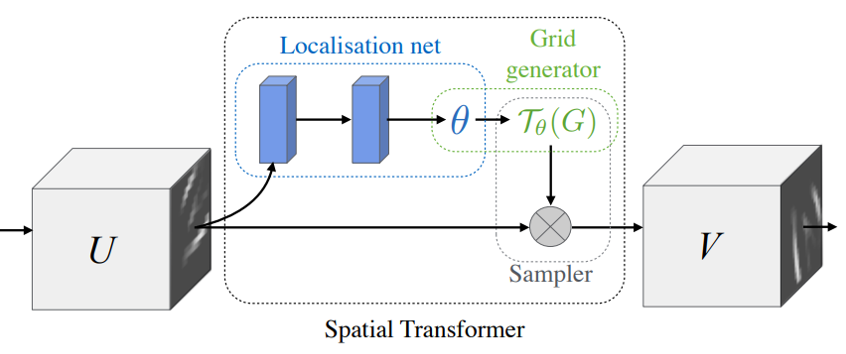
\includegraphics[width=\linewidth]{images/01_ST.PNG}
 \textbf{Localization Network} 간단한 구조로 일종의 neural network이다. 좌표를 transform 해주기 위한 parameter $\theta$ 을 찾아준다.
 제약 조건은 마지막 단에 regression layer가 필요하다. $ \theta = f_{loc}(U)$ 로 식을 쓸 수가 있다.
 \newline  \textbf{Parameterized Sampling Grid:gird generator} 여기에서는 parameter $\theta$를 가지고 input image와 output image 사이의 좌표를 변환해주는
 grid를 계산해준다. 아래그림을 보면 좀더 명확하다. 왼쪽 그림은 identity transformation, 오른쪽 그림은 affine transform을 나타낸다. 
 이 그림을 보고 설명하자면 identity transformation에 경우에는 input의 pixel을 그대로 반영해서 output으로 내보내는 것을 볼 수 있다. 반면
 affine transform의 경우에는 input pixel에서 공간적인 변형을 적용시켜줘서 output pixel에 대응하도록 설계되어있다.
 \newline  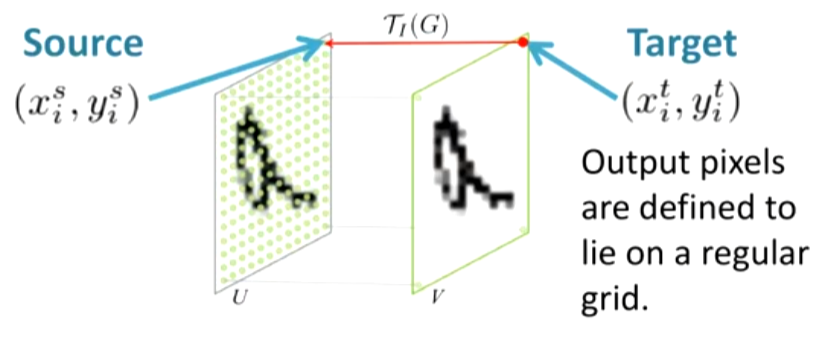
\includegraphics[width=5cm, height=3cm]{images/02_ST.PNG} 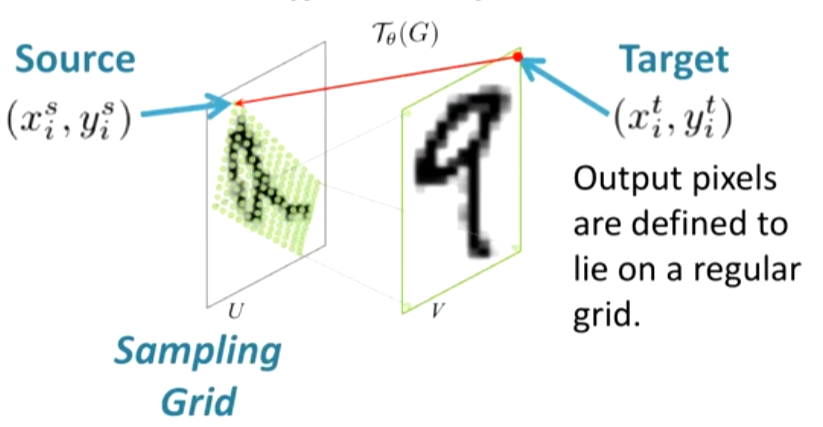
\includegraphics[width=5cm, height=3cm]{images/03_ST.PNG}
 \newline affine transform은 공간을 변형하는 것으로 이해하면 되는데 예를 들면
 scale, rotation, translation, skew, cropping 이 있다. 6가지의 parameter을 가지고 있으며 아래 그림과 같이 변형이 일어난다. Localization Network에서 $\theta$의 값을 찾고
 gird generator에서는 input data의 pixel 옮기는 것이다. 
 \newline  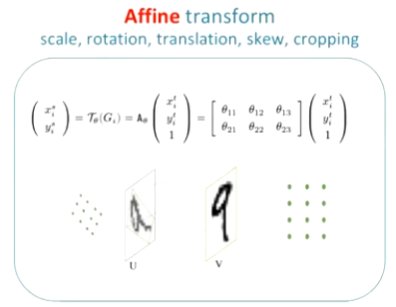
\includegraphics[width=7cm, height=4cm]{images/04_ST.PNG}
 \newline attention의 경우에는 isotropic scale을 의미하는 것으로 4개의 parameter만을 가지고 있다. \cite{youtube}
 \newline  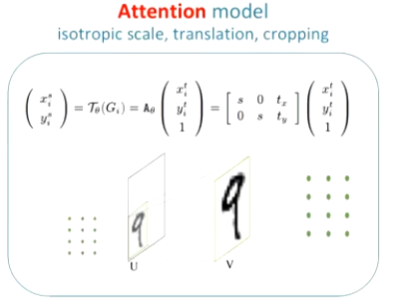
\includegraphics[width=7cm, height=4cm]{images/05_ST.PNG}
 \newline \textbf{Differentiable Image Sampling : Sampler} 위의 localization network와 gird generator의 결과를 받아서 input point를 output point로 mapping 시켜준다.
 즉 gird generator가 발생시킨 좌표값을 하나씩 mapping 시켜주면 된다. 여기서 고려할 문제가 interpolation이다. sampling kernel을 generic하게 modeling하면 아래와 같은 형태로 나타난다.
 \newline  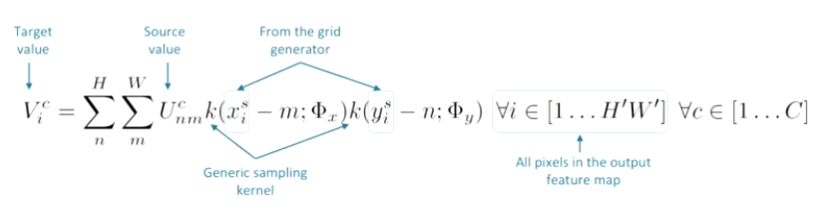
\includegraphics[width=\linewidth]{images/06_ST.PNG}
 예를 들어보자면 가까운 pixel을 읽어오고 싶다면 integer sampling을 진행하면 되므로 아래와 같은 식을 사용할 수 있다.
 \newline  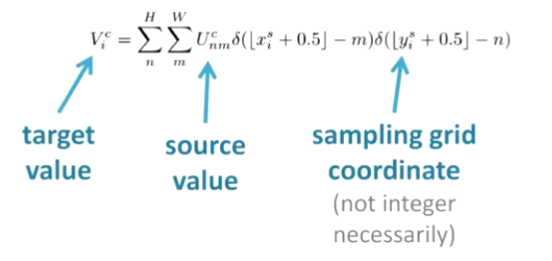
\includegraphics[width=7cm, height=3cm]{images/07_ST.PNG}
 \newline x,y축으로 각각 linear interpolation을 해주는 bilinear sampling을 가장 많이 사용하고 필요에 따라 중간값을 sampling하도록 설계하면 된다. 
 아래는 original image을 각기 다른 방법으로 sampling한 결과이다. 
 \newline  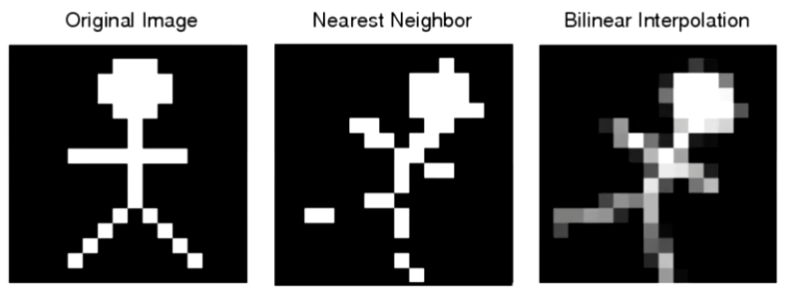
\includegraphics[width=7cm, height=3cm]{images/08_ST.PNG}
 \newline  target value를 미분 가능하게 설계하면 loss function을 별도로 설계하지 않아도 CNN으로 부터 backpropagation이 진행되는 동안 함께 학습이 가능하다.
 \newline \textbf{Spatial Transformer Networks} 이 ST(spatial transformer) module은 여러개 삽입해도 된다. 만약 병렬로 삽입하게 된다면 다중 물체가 있는 그림에 각각 focus하겠다는 의미가 된다.
 
 \subsection{Experiments}
 \textbf{Distorted versions of the MNIST handwriting dataset for classification} 이 실험은 변형시킨 MNIST dataset을 가지고 실험을 진행하는 것으로 rotation, rotation, scale-translation(RTS), projective, elastic
 의 방법으로 변형시킨다. 아래 오른쪽 그림을 보면 변형된 input data의 변형을 잘 detect하여 ST module을 통과시킨 새로운 CNN에 들어갈 input data가 regular함을 확인할 수 있다.
 \newline  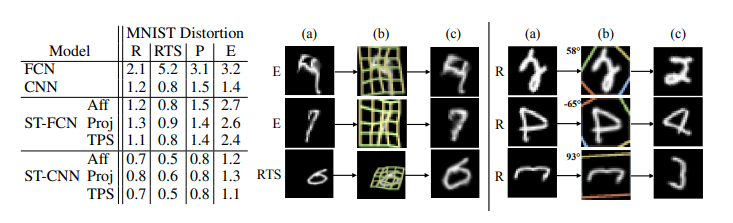
\includegraphics[width=\linewidth]{images/09_ST.PNG}
  ST(spatial transformer) module를 삽입한 결과가 기존 CNN 결과보다 더 좋다. 또한 FCN에 삽입한 것보다 CNN에 삽입한게 결과가 좋았는데 원래 FCN보다 CNN의 성능이 좋기도 하고 
  CNN에서는 2개의 pooling layer가 있기 때문에 ST와 상호보완적으로 공간적 변형을 인식하는 효과가 있다. sampling의 경우 bilinear sampling으로 통일했지만, transformation function은 
  affine, projection, 16개의 parameter을 가지고 있는 thin plate spline transformation 각각 사용했다고 한다.
 아래 그림은 spatial transformer을 2개를 넣은 것으로 각 channel에 independent하게 ST module이 학습됨을 의미한다. 
 \newline  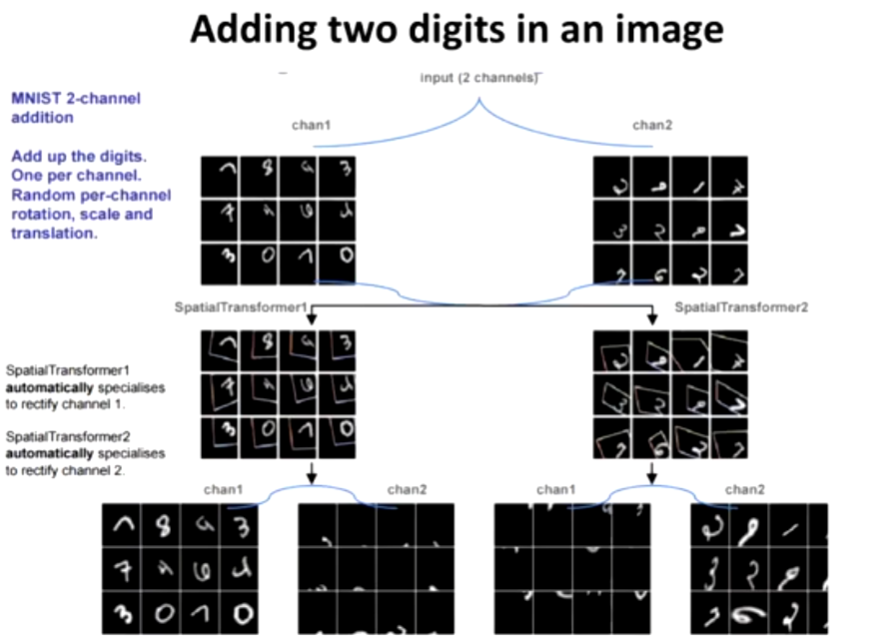
\includegraphics[width=10cm, height=6.5cm]{images/10_ST.PNG}
 자세한 영상은 다음 사이트를 참고하자.
 \href{https://www.youtube.com/watch?v=yGFVO2B8gok&t=8s}{DeepMind}
 \newline \textbf{A challenging real-world dataset, Street View House Numbers for number recognition}
 이 실험은 각각의 이미지에서 sequence of numbers,1 $\sim$ 5개 사이의 digits으로 이루어진 데이터를 인식하는 것으로 실제 데이터이기 때문에 매우 scale이 다양하고 
 공간적 배열도 다양하게 되어 있다. 전처리로 이미지 주변의 64x64 crop을 하거나 128x128 crop을 진행하였다. 또한 5개의 독립적인 softmax classifier이 몇자리수인지 판단한다.
 이 실험에는 CNN 들어가기전 module을 삽입하기도 했지만 더 깊은 곳에서 module을 삽입하였는데 그 결과 중간 중간 feature map에서도 공간적인 정보 변형을 일반화해줄 수 있었다.
 하지만 거의 정확도 차이가 없기 때문에 computation seed가 더 느린만큼 single을 사용해도 충분할 것 같다.(speed는 single과 multi는 거의 차이가 없다. 왜냐하면 module이 너무 간단하기 때문이다.
 실제로 multi ST-CNN과 CNN을 비교하면 6\%정도 차이가 난다고 실험 결과에서 밝힌다.)
 \newline  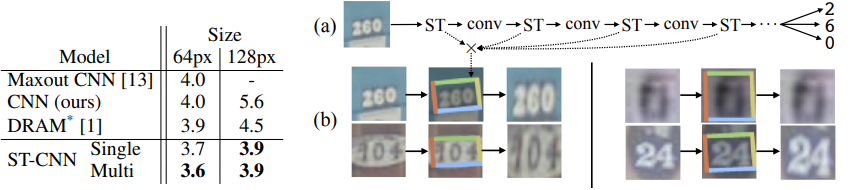
\includegraphics[width=\linewidth]{images/11_ST.PNG}
 \newline \textbf{CUB-200-2011 birds dataset for fine-grained classification by using multiple parallel spatial transformers}
 실험 결과가 특별한데 아래 그림을 보면 알 수 있듯이 parallel로 ST module을 쌓은 경우에 각각의 module은 다른 곳을 집중해서 보는 것을 확인할 수 있다.
 빨간색을 보면 새의 머리 주변을 보고 초록색박스는 몸통의 중심을 기준으로 crop된 image을 집중하는 것을 볼 수 있다. 이 실험에 대해서 간략히 말하자면 inception model에다가
 ST module을 삽입하였다. 이 실험으로 알 수 있는 것은 원래 이미지의 크기가 있으면 ST module을 이용해서 성능의 하락없이 이미지를 적절히 downsampling이 가능하다는 것이다.
 또한 결과의 box를 보면 알 수 있듯이 사물 detection의 효과도 있는 것을 확인할 수 있다.
 \newline  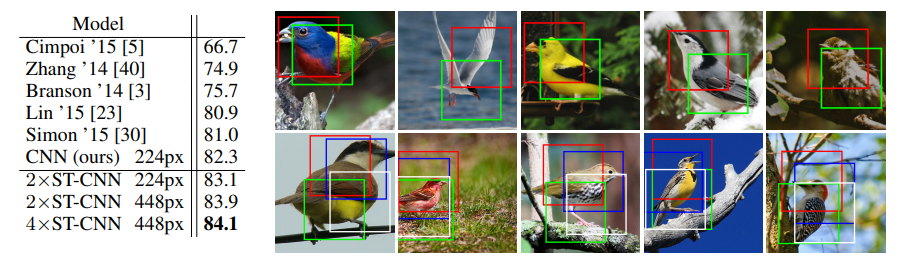
\includegraphics[width=\linewidth]{images/12_ST.PNG}
\subsection{Conclusion}
 이 논문에서는 neural network에 적용가능한 새로운 self-contained module(ST)을 소개하였다. 이 module은 간단히 기존 알고리즘에 삽입하여(보통 input단에 삽입하는 것이 사람이 해석하기에 더 효과가 있다.) 
 사용할 수 있고 또한 별도의 loss function의 변화없이 미분가능한 module이기 때문에 end to end 학습이 가능하다. 또한 3D transformation에도 쉽게 확장 가능하다.
\newpage
\bibliography{egbib}

\end{document}
